\chapter{Divergencia e integral de Skorokhod}

\begin{definicion}
El operador divergencia $\dive$ es el adjunto de $\D$: $u\in L^2(\Omega;\Hil)$ está en
$\operatorname{Dom}\dive$ si $|\E\ip{\D F}{u}|\le c\norm{F}_{L^2}$ para toda $F\in\mathcal S$, y entonces
\begin{equation}\label{eq:ibp}
  \E\big[\ip{\D F}{u}\big]=\E\big[F\,\dive(u)\big].
\end{equation}
\end{definicion}

\begin{proposicion}
\begin{enumerate}
  \item Si $h$ es determinista, $\dive(h)=W(h)$.
  \item Si $u$ es adaptado y de cuadrado integrable, $\dive(u)=\int_0^Tu_t\dd W_t$ (Itô).
  \item Si $G\in\Dom$ y $Gu\in\operatorname{Dom}\dive$: $\dive(Gu)=G\dive(u)-\ip{\D G}{u}$.
\end{enumerate}
\end{proposicion}

Por (2), $\dive$ extiende la integral de Itô a integrandos anticipativos: es la
integral de Skorokhod \cite{skorokhod1975}.

\begin{ejemplo}
Con $u_t=W_T$ (no adaptado), por (3): $\dive(W_T)=W_TW_T-\ip{\ind}{\ind}=W_T^2-T$.
Tomando $F=W_T^2$ en \eqref{eq:ibp}: $\E[2W_T\cdot W_T\cdot T]=2T^2=\E[W_T^2(W_T^2-T)]$.
\end{ejemplo}

\paragraph{Lema clave para finanzas.} Si $\ip{\D F}{u}\neq0$ c.s., aplicando
\eqref{eq:ibp} a $\varphi(F)$ con integrando $u/\ip{\D F}{u}$:
\begin{equation}\label{eq:peso}
  \E[\varphi'(F)G]=\E\Big[\varphi(F)\,\dive\Big(\frac{G\,u}{\ip{\D F}{u}}\Big)\Big].
\end{equation}

\begin{figure}[h]
  \centering
  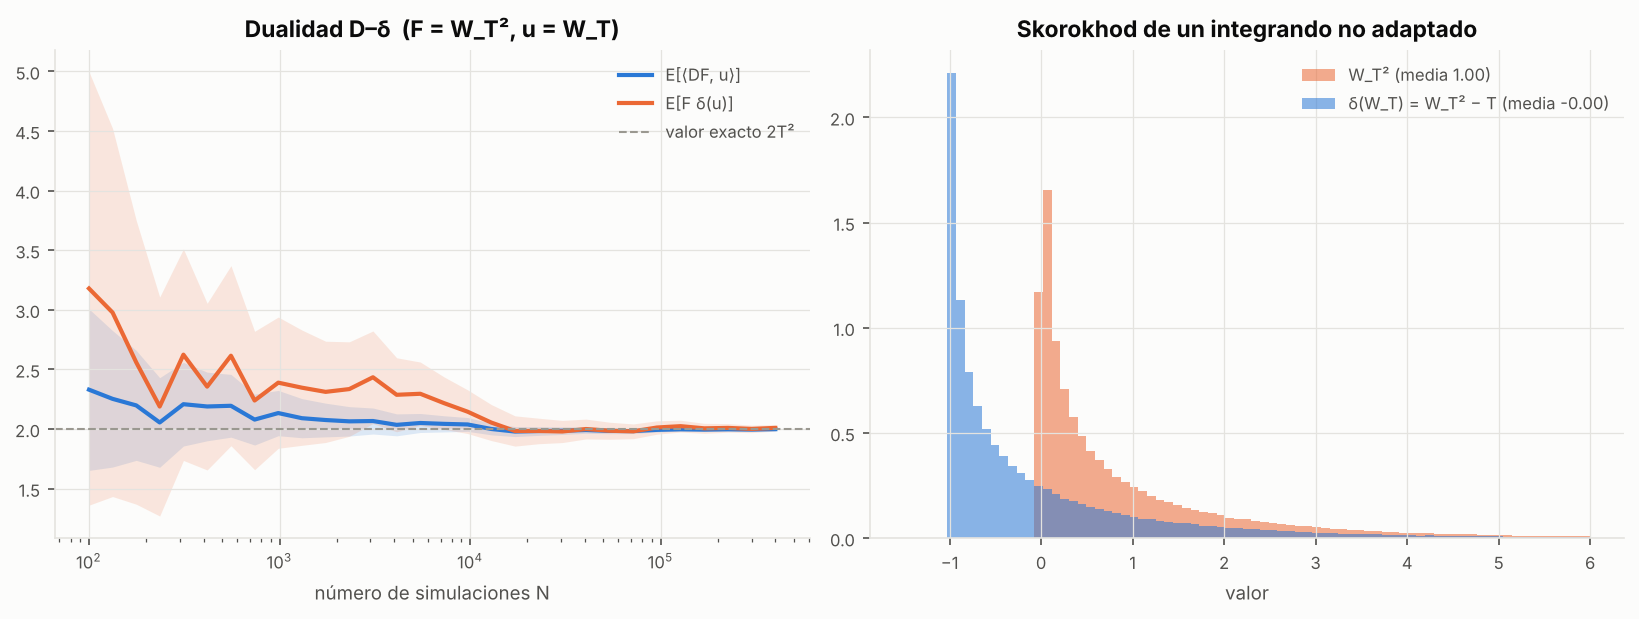
\includegraphics[width=0.95\linewidth]{03_integracion_por_partes}
  \caption{Verificación Monte Carlo de la dualidad y comparación
  $\dive(W_T)$ vs.\ $W_T^2$ (\codigo{examples/03\_integracion\_por\_partes.py}).}
\end{figure}
